\documentclass[tikz, border=10pt]{standalone}
\usepackage{pgfplots}
\pgfplotsset{compat=1.18}
\usepackage{amsmath}
\begin{document}
	
	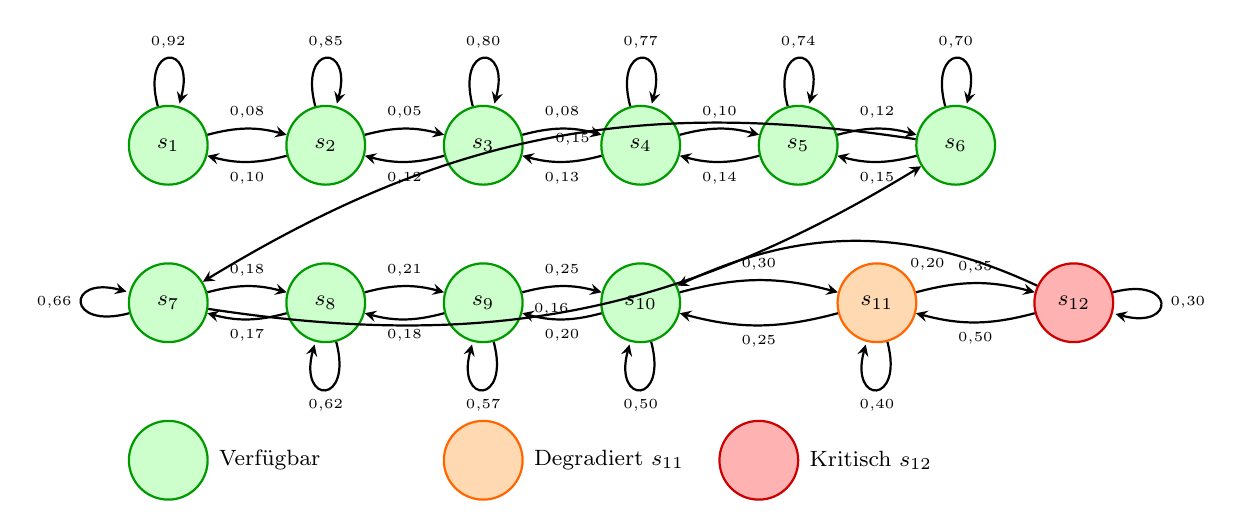
\begin{tikzpicture}[->, >=stealth, node distance=2cm, thick]
		\tikzstyle{available}=[circle, draw=green!60!black, fill=green!20, minimum size=1cm, font=\footnotesize]
		\tikzstyle{degraded}=[circle, draw=orange!80!red, fill=orange!30, minimum size=1cm, font=\footnotesize]
		\tikzstyle{critical}=[circle, draw=red!80!black, fill=red!30, minimum size=1cm, font=\footnotesize]
		
		% Zustände s1 bis s10 in zwei Reihen anordnen
		% Obere Reihe: s1 bis s6
		\node[available] (s1) at (0,2) {$s_1$};
		\node[available] (s2) at (2,2) {$s_2$};
		\node[available] (s3) at (4,2) {$s_3$};
		\node[available] (s4) at (6,2) {$s_4$};
		\node[available] (s5) at (8,2) {$s_5$};
		\node[available] (s6) at (10,2) {$s_6$};
		
		% Untere Reihe: s7 bis s10
		\node[available] (s7) at (0,0) {$s_7$};
		\node[available] (s8) at (2,0) {$s_8$};
		\node[available] (s9) at (4,0) {$s_9$};
		\node[available] (s10) at (6,0) {$s_{10}$};
		
		% Degradiert und kritisch
		\node[degraded] (s11) at (9,0) {$s_{11}$};
		\node[critical] (s12) at (11.5,0) {$s_{12}$};
		
		% Übergänge obere Reihe (s1 bis s6)
		\draw (s1) edge[loop above] node[above, font=\tiny] {$0{,}92$} (s1);
		\draw (s1) edge[bend left=15] node[above, font=\tiny] {$0{,}08$} (s2);
		
		\draw (s2) edge[bend left=15] node[below, font=\tiny] {$0{,}10$} (s1);
		\draw (s2) edge[loop above] node[above, font=\tiny] {$0{,}85$} (s2);
		\draw (s2) edge[bend left=15] node[above, font=\tiny] {$0{,}05$} (s3);
		
		\draw (s3) edge[bend left=15] node[below, font=\tiny] {$0{,}12$} (s2);
		\draw (s3) edge[loop above] node[above, font=\tiny] {$0{,}80$} (s3);
		\draw (s3) edge[bend left=15] node[above, font=\tiny] {$0{,}08$} (s4);
		
		\draw (s4) edge[bend left=15] node[below, font=\tiny] {$0{,}13$} (s3);
		\draw (s4) edge[loop above] node[above, font=\tiny] {$0{,}77$} (s4);
		\draw (s4) edge[bend left=15] node[above, font=\tiny] {$0{,}10$} (s5);
		
		\draw (s5) edge[bend left=15] node[below, font=\tiny] {$0{,}14$} (s4);
		\draw (s5) edge[loop above] node[above, font=\tiny] {$0{,}74$} (s5);
		\draw (s5) edge[bend left=15] node[above, font=\tiny] {$0{,}12$} (s6);
		
		\draw (s6) edge[bend left=15] node[below, font=\tiny] {$0{,}15$} (s5);
		\draw (s6) edge[loop above] node[above, font=\tiny] {$0{,}70$} (s6);
		
		% Verbindung von s6 zu s7 (Übergang zur unteren Reihe)
		\draw (s6) edge[bend right=20] node[right, font=\tiny] {$0{,}15$} (s7);
		
		% Übergänge untere Reihe (s7 bis s10)
		\draw (s7) edge[bend right=20] node[left, font=\tiny] {$0{,}16$} (s6);
		\draw (s7) edge[loop left] node[left, font=\tiny] {$0{,}66$} (s7);
		\draw (s7) edge[bend left=15] node[above, font=\tiny] {$0{,}18$} (s8);
		
		\draw (s8) edge[bend left=15] node[below, font=\tiny] {$0{,}17$} (s7);
		\draw (s8) edge[loop below] node[below, font=\tiny] {$0{,}62$} (s8);
		\draw (s8) edge[bend left=15] node[above, font=\tiny] {$0{,}21$} (s9);
		
		\draw (s9) edge[bend left=15] node[below, font=\tiny] {$0{,}18$} (s8);
		\draw (s9) edge[loop below] node[below, font=\tiny] {$0{,}57$} (s9);
		\draw (s9) edge[bend left=15] node[above, font=\tiny] {$0{,}25$} (s10);
		
		\draw (s10) edge[bend left=15] node[below, font=\tiny] {$0{,}20$} (s9);
		\draw (s10) edge[loop below] node[below, font=\tiny] {$0{,}50$} (s10);
		\draw (s10) edge[bend left=15] node[above, font=\tiny] {$0{,}30$} (s11);
		
		% Übergänge zu degradiert und kritisch
		\draw (s11) edge[bend left=15] node[below, font=\tiny] {$0{,}25$} (s10);
		\draw (s11) edge[loop below] node[below, font=\tiny] {$0{,}40$} (s11);
		\draw (s11) edge[bend left=15] node[above, font=\tiny] {$0{,}35$} (s12);
		
		\draw (s12) edge[bend left=15] node[below, font=\tiny] {$0{,}50$} (s11);
		\draw (s12) edge[bend right=25] node[below, pos=0.3, font=\tiny] {$0{,}20$} (s10);
		\draw (s12) edge[loop right] node[right, font=\tiny] {$0{,}30$} (s12);
		
		% Legende
		\node[available, label=right:{\footnotesize Verfügbar}] at (0,-2) {};
		\node[degraded, label=right:{\footnotesize Degradiert $s_{11}$}] at (4,-2) {};
		\node[critical, label=right:{\footnotesize Kritisch $s_{12}$}] at (7.5,-2) {};
		
	\end{tikzpicture}
	
\end{document}